% TODO pas sur mais ca peux etre sympa si on se focus plus a cheerios que ceci est pour un cours peut etre ? je sais pas ? qui sais ? pas moi en tot cas. 
On a tous mange des ceriales ou vu des objets flottant atirer vers ou pouse par eux; mais cest quoi la raison de cette force dans ce projet cree au sein de l'UE projet en calcul scientific on a fait la simulation des objets flottants.

TODO faire un tableau de symboles que on utilise comme \(\gamma\) surface tension etc

\begin{table}
    \centering
    \begin{tabular}{ccc}
        \hline
        abraviation & nom & dimension\\
        \hline
        $R$      & Rayon de courbure & TODO\\
        $\gamma$ & surface tension   & TODO\\ 
        $\rho_s$ & densite solide    & TODO\\
        $\rho_l$ & densite liquide   & TODO\\
        $\rho_a$ & densite air       & TODO\\
        $B$      & nombre de Bond    & TODO\\
        \hline
    \end{tabular}
    \caption{Table des variables}
\end{table}

\subsection{Effet Cheerios}
    Cette partie est plutot fait pour lintegrite du rapport le lecteur est fortement encourage a lire \cite{vella_cheerios_2005} pour avour une plus complete comprehension du sujet \textit{cheerios effect}
    Les formules pour les calculs viennent principalement de \cite{vella_cheerios_2005}
    TODO expliquer de ou viens les forces des angles qui tord la surface ?

    Expliquer leffet de cheerios.
    
    % TODO peut etre notre propre figure ?
    \begin{figure}
        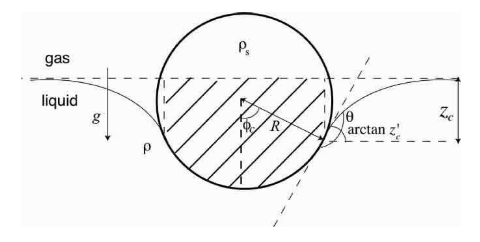
\includegraphics[width = 0.9\textwidth]{boulleflotantedecheerios.png}
        \caption{Geometry of a sphere lying at a liquid-gas interface. The shaded area represents the weight of liquid equivalent to the buoyancy force due to hydrostatic pressure acting on the sphere.\cite{vella_cheerios_2005}}
    \end{figure}
    Une des raisons la quel les objets flotte cest due a la pusee de archimede et ces't un des cas majeurs dans notre probleme aussi. Comme on peux voir dans la figure TODO metre la citation de la figure en haut.
    
    Pour que notre sphere reste sur linterface il a besoin que son poids \(\frac{4}{3}\pi\rho_{s}gR^3\) devrait etre en equilibre par la composante de pousee de archimede a lendroit de contact du liquide avec la sphere et la force de tension sur la surface ??? must be balanced by the component of surface tension acting along the (circular) contact line and the buoyancy force because of the displaced bulk fluid.

    TODO expiquer dou ca viens moi ja pas comprie
    \begin{equation}
        2\pi R \phi_c \gamma \sin(\arctan z_c^{'}) = 2\pi\gamma R \sin\phi_c z_c^{'}(1+z_c^{'2})^{-1/2}
        \label{eq:wut}
    \end{equation}

    Buoyancy force
    \begin{equation}
        \pi\rho_l g R^3 (\frac{z_c}{R}\sin^2 \phi_c + \frac{2}{3}-\cos\phi_c+\frac{1}{3}\cos^3 \phi_c)
        \label{eq:buoyancyForce}
    \end{equation}

    Balance of vertical forces
    Alors on a
    \begin{equation}
        \Rightarrow \frac{4}{3}\pi\rho_{s}gR^3 =2\pi\gamma R \sin\phi_c \frac{z_c^{'}}{\sqrt{(1+z_c^{'2})}} + \pi\rho_l g R^3 (\frac{z_c}{R}\sin^2 \phi_c + \frac{2}{3}-\cos\phi_c+\frac{1}{3}\cos^3 \phi_c)
    \end{equation}

    TODO cest quoi $z_c^{'}$???

    Si on substitue \(\phi_c = \pi - \theta + \arctan z_c^{'}\) et garde seulement les termes linear en \(z_c^{'}\) on retrouve l'expression pour \(z_c^{'}\sin \phi_c\) qui est precis a \textit{linear order in the Bond number} \(B \equiv R^2/L_c^2\) 

    Alors on a:
    \begin{equation}
        z_c^{'}\sin \phi_c = B(\frac{2D-1}{3}-\frac{1}{2}\cos \theta + \frac{1}{6} \cos^3 \theta) \equiv B\Sigma
        \label{eq:bondsigma}
    \end{equation}
    Avec \(D \equiv \rho_s / \rho\) On peux voir ceci est bien le cas car on observe bien que \(z_c^{'} = 0\) quand \(\theta = \pi/2\) et \(D = 1/2\) cest ce que on satendais car dans ce cas la pousee de archimede seul lui meme est assez pour equilibrer le poids de la sphere sans deformations du liquide.

    L'equation\ref{eq:bondsigma}contient deux parametres sans dimensions; \textit{Bond number}$B$ et $\Sigma$ tres importants pour notre modélisation.

    \begin{equation}
        B = \frac{(\rho_l-\rho_{a})gR^2}{\gamma}
    \end{equation}
    Le nomre de Bond nous donne la mesure relative de limportance des effets de gravite et tension de surface; si $B$ est tres grande ca correspond a des particules grandes ou une tension de surface petit. 

    WUT ????

    The expression for the slope of the interface in the vicinity of the spherical particle given in (9) is valid for B << 1 (corresponding to a radius of  1mm or smaller for a sphere at an air-water interface) in which case surface tension is very important. The other dimensionless parameter, , can be thought of as a (non-dimensional) resultant weight of the particle once the Archimedes upthrust has been subtracted out. This physical interpretation arises naturally from the vertical force balance condition (8) and (9) since the resultant weight of the object (in the linearised approximation) is simply 

    To calculate the interaction energy using the Nicolson
    approximation, we must also calculate the interfacial displacement caused by an isolated floating sphere, which is determined by the hydrostatic balance gamma nabla²h = rho gh - the co-ordinate invariant statement of equation (1). With the assumption of cylindrical symmetry, this becomes:
    \(\gamma \nabla^2h = \rho_l g h\)
    \begin{equation}
        \gamma \frac{\dd^2h}{\dd x^2} = \rho_l g h
    \end{equation}
    Si on assume une symetrie spherique
    \begin{equation}
        \Rightarrow \frac{1}{r} \frac{\dd}{\dd r} \left( r\frac{\dd h}{\dd r}\right) = \frac{h}{L_c^2}
    \end{equation}
    TODO developer bessel
    \cite{introtoBessel}

    % TODO dans le code ajouter un buoyancy force qui calcule la ousee de archimede et dis si notre objet flotte ou pas si il flotte pas on peux metre un option tel quel il prend la valeur automatique ??? Ou on le neglige ????
    % TODO On mets les formules et peut etre demontrer ou ils viennent et surtout les cas ou on peux utiliser ces formules les cas ou ca marche pas etc\ldots
    % TODO SCHEMA deux cheeios et sur le schema on monre l Rayon de courbure etc...
    % TODO graphique des foncions de bessel
    % TODO citer cheerios 
    \begin{equation}
        \label{ForceEntreCheerios}
        F(l) = -2\pi \gamma R B^{5/2} K_1 \left( \frac{l}{L_c}\right)
    \end{equation}
